\documentclass[titlesmallcaps, examinerscopy, copyrightpage]{uqthesis}

\bibliographystyle{customIEEEtran}

\usepackage[usenames,dvipsnames]{color}
\usepackage[square,comma,numbers,sort&compress]{natbib}
\usepackage{pdfpages}
\usepackage{graphicx}
\usepackage{eurosym}
\usepackage{appendix}
\usepackage{play}
\usepackage[grey,times]{quotchap}
\usepackage{makeidx}
\makeindex
\usepackage{hyperref}
\usepackage{listings}
\usepackage[nottoc,numbib]{tocbibind}
\usepackage{verbatim}
\usepackage{amsfonts}
\usepackage{array}
\usepackage[acronym,nomain,nonumberlist]{glossaries}
\usepackage{listings}
\usepackage{setspace}
\usepackage[linewidth=1pt]{mdframed}
\usepackage{sverb}
\usepackage{bookmark}
\bookmarksetup{
  numbered, 
  open,
}

\makeglossaries
\renewcommand*{\glossaryentrynumbers}[1]{}

\newcommand{\tick}{\checkmark}
\newcommand{\gtick}{\color{ForestGreen} \tick }
\newcommand{\cross}{$\times$ }
\newcommand{\rcross}{\color{red} \cross }


\begin{document}
% =====================================================================
% =====================================================================
%%%%%%     TITLE
% =====================================================================
% =====================================================================

\hypersetup{pageanchor=true}
\pdfbookmark{Title}{toc}

\title{Undergraduate Thesis\\ \vspace{0.5 cm} ``Automatic and Assisted Redshift Analysis of Astronomical Objects" }
\author{Samuel Hinton}
\department{EAIT}

\renewcommand{\degreetext}{in partial fulfilment of the Degree Bachelor of Engineering\\ in the
discipline of Software Engineering}

\frontmatter

\titlepage



% =====================================================================
% =====================================================================
%%%%%%     FRONT CONTENT
% =====================================================================
% =====================================================================

\begin{flushright}
Samuel Hinton\\ 42345493\\ 78 Pegg Road, Rocklea, QLD 4106\\
\end{flushright}

\noindent \today \\

\noindent Prof Paul Strooper\\
Head of School\\
School of Information Technology and Electrical Engineering\\
The University of  Queensland\\
St Lucia QLD 4072\\

\noindent Dear Professor Strooper,\\ \\
In accordance with the requirement of the Degree of Bachelor of Engineering (Honours) in the School
of Information Technology and Electrical Engineering, I submit the following thesis entitled:

\begin{center}
  \emph{``Automatic and Assisted Redshift Analysis of Astronomical Objects''}
\end{center}

\noindent The thesis was performed under the supervisor of Dr Vaughan Clarkson and Dr Tamara Davis. I declare that the work
submitted in thesis is my own, except as acknowledge in the text and footnotes, and has not been
previously submitted for a degree at the University of Queensland or any other institution. \\

\noindent Yours sincerely \\ \\ 

\noindent \line(1,0){250} \\

\noindent Samuel Hinton

% =====================================================================

\chapter{Acknowledgements}

I would like to thank my supervisors, Tamara Davis, Vaughan Clarkson and Chris Lidman for their help, assistance and guidance throughout this thesis. I would also like to thank David Parkinson, Conor O'Neill, Michael Childress, David Lagattuta, Syed Uddin, Fang Yuan, Jeremy Mould, Richard Scalzo, Anthea King, Bonnie Zhang and Karl Glazebrook for their feedback, suggestions and testing during this thesis.

% =====================================================================

\chapter{Abstract}

I AM THE ABSTRACT


\cleardoublepage
\hypersetup{pageanchor=true}
\pdfbookmark[chapter]{Table of Contents}{toc}
%\addcontentsline{toc}{chapter}{Table of Contents}

\tableofcontents
\listoffigures
\listoftables

%\printglossary[title=Glossary]
%\addcontentsline{toc}{chapter}{Glossary}

\mainmatter


\chapter{Introduction}

Redshifting measurements form the backbone of many cosmological surveys, and in order to turn spectrographic measurements into quantified redshifts, a redshifting program is needed. In this thesis, the legacy redshifting software used by the OzDES cosmology team, RUNZ, is replaced with a new, web-based redshifting application developed specifically for their needs of high redshift and low signal-to-noise algorithms.\\

This report is divided into several sections, with the background and context for redshifting established in Chapter \ref{ch:back} and prior implementations discussed in Chapter \ref{ch:prior}. Those familiar redshifting and prior approaches are recommended to read from Chapter \ref{ch:req} or Chapter \ref{ch:impl}, where program requirements and the implementation results are respectively discussed.



\chapter{Background}
\label{ch:back}

\section{Usefulness}

Redshifting a spectra is the process by which the degree of spectra from its original emission state is quantified. Over cosmic distances, the expansion of the universe causes travelling light to become stretched, and thus the measured amount of stretching provides valuable information about the travel time of the light, and thus the distance to the emission entity. As multiple cosmological models are still being actively considered \cite{davis2007scrutinizing}, it is prudent to keep measurements in the form of redshifts, as different cosmological models will translate redshifts to different comoving distances.\\

Redshifting can be obtained both from spectrographic and photometric data, each with advantages and disadvantages. Whilst photometric data can be used for fainter objects than currently viable for spectrographs, photometric redshifts do not possess the accuracy of spectrographic measurements \cite{bolzonella2000photometric}. It is important to note that the OzDES team, for which this thesis was undertaken, are not utilising any photometric redshifts as priors, nor does their instrumentation require photometric data. The OzDES team are utilising the Anglo-Australian Telescope (AAT) with the AAOmega spectrograph \cite{d2014ozdes}, and thus only require a spectrographic redshifting solution.

\section{Spectrographic Features}

Spectrographs provide accurate redshifting due to prominent discernible features in light emissions for galactic objects, where abundant elements such as Hydrogen, Nitrogen and Carbon either emit or absorb at different frequencies. Provided a high enough signal-to-noise ratio in a spectra, these peaks and troughs can be identified as potential features. Provided a sufficient amount of features, and they can be matched to known atomic transitions, whereupon the observed feature wavelength and the known feature wavelength can be combined to determine the redshift of a spectra. Figure \ref{fig:emission} provides a visual example of a high signal-to-noise spectra of the Seyfert 2 galaxy NGC 1068 (M77).

\begin{figure}[ht!]
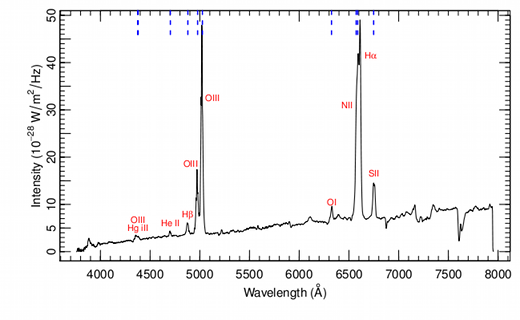
\includegraphics[width=0.75\textwidth]{images/M77_opt_spectrum.png} 
\centering
\caption{A plot of the emission from NGC 1068, with data from the NASA/IPAC Extragalactic Database\cite{nasaDB} and plot courtesy of public R code published by Alastair Sanderson \cite{emission}.}
\label{fig:emission}
\end{figure}

\section{Common Complications}

High quality spectra, with well defined and multiple emission features, such as shown in Figure \ref{fig:emission}, become progressively less common with increasing redshift, due to increasing distance to emission object and thus lower light intensity. As such, redshifting algorithms have to employ data reduction and matching techniques specifically designed to marginalise potential error and account of known complications. In this section, several complications to the redshifting process that have been actively encountered in this thesis will be discussed. Ideas on how to marginalise or reduce these complications will be discussed in the implementation section of this thesis.

\subsection{Planetary Atmospheric Interference}

Given that the Anglo-Australian Telescope is located on the ground in Australia, interference from the night sky has to be dealt with. The sky itself, possessing both necessary ingredients of light and atoms, has its own emission spectrum which all spectrographs will detect \cite{Meinel1950Emission}. By observing the night sky without a background source, the night sky can be subtracted out of target spectra, however this process can be imperfect in implementation due to spectrograph error and optical distortion \cite{Kelson2003Optimal}. Figure \ref{fig:night} shows the night sky spectrum above Mauna Kea.

\begin{figure}[ht!]
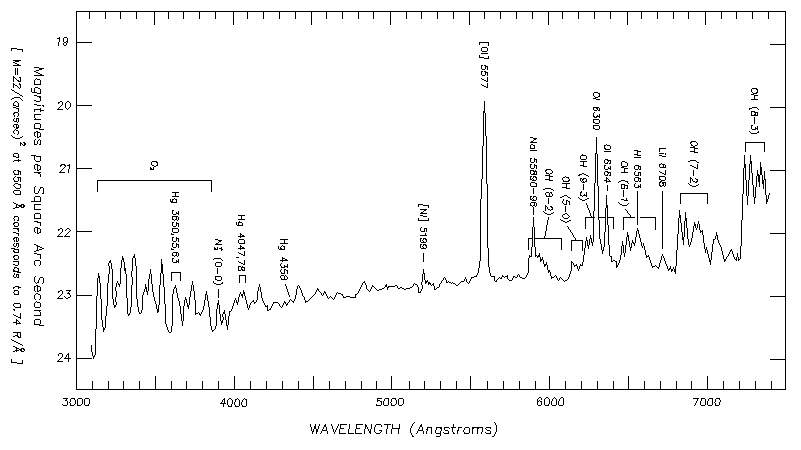
\includegraphics[width=0.75\textwidth]{images/om-nskyvis.jpg} 
\centering
\caption{A plot of the night sky emission above Mauna Kea from the Canada-France-Hawaii Telescope Observatory Manual \cite{night}. Please see the manual for data sources and further attribution.}
\label{fig:night}
\end{figure}

\subsection{Planetary Atmospheric Correction}

A simple consideration when examining spectra is that the wavelengths being recorded are the wavelengths of light in air (for a ground based telescope). Due to the complicated nature of converting air wavelengths to vacuum wavelengths, this is often done via interpolating conversions from empirical tabular data sets \cite{morton1991atomic}.

\subsection{Heliocentric velocity}

With the accuracy of spectrographic redshifting, the planet's heliocentric velocity provides a significant enough contribution that it needs to be corrected for \cite{colless20012df,baldry2014galaxy}. This can be done by calculating the relative velocity of the Earth in its solar orbit relative to the object being observed, and subtracting the appropriate redshift contribution.

\subsection{Cosmic Rays}

Cosmic rays are the name given to extremely high energy particles travelling in space. Cosmic rays are generally massive particles such as protons moving at relativistic speeds, often due to acceleration in a supernova \cite{ackermann2013detection}. Due to their colossal energy, in which the record is approximately $3\times10^{8}$ TeV (23 million times as energetic as the maximum energy rating of the Large Hadron Collider when set to reopen in 2015 \cite{lhc}), a single strike by a cosmic ray will appear as an extraordinarily thin and powerful emission line in a spectrum. Difficulty arises in filtering out cosmic ray strikes, but not filtering out emission lines, as the two features are similar in a spectra.

\subsection{Equipment Miscalibration}

Talk about spectral arms


\subsection{Non-uniform spectroscopic sensitivity}

Talk about that stuff

\chapter{Prior Methods}
\label{ch:prior}

Brief intro. Talk about how the differences in data and files for each telescope and specrograph have meant individualised software.
\section{Implementations}

\subsection{RVSAO 2.0}

\subsection{2dF Galaxy Redshift Survey}

\subsection{SDSS DR8 $\chi^2$ fitting}

\subsection{AUTOZ}

\section{Trends and Caveats}

% =====================================================================

\chapter{Requirements}
\label{ch:req}

Requirements.

\section{Algorithm Performance}

Has to be better than Runz

\section{Computational Performance}

Has to run. Time not too much of an issue.

\section{Usability}

Talk about install problems, updates, making it quick and easy to use. Introduce the novel concept of scientific computing.

\chapter{Implementation}
\label{ch:impl}

Talk about EVERYTHINGGGGGGG



\chapter{Project Evaluation}

\section{Completion}



\begin{table}[ht!]
	\center
	\begin{tabular}{c|c|c}
		\hline
		Feature & Complete & Incomplete \\
		\hline
		Surface Capture & \gtick & \\
		Human interface (Control Panel) & \gtick & full UI synchronisation between multiple clients \\
		External control interface (RPC) & \gtick & \\
		Configurable (JSON Keystore) & \gtick & More settings should be user configurable \\
		Real-time Computer Vision for \newline Block Diagram recognition & \gtick & \\
		Block Diagram Model output \newline (MQTT Publish/Subscribe) & \gtick & \\
		\ldots & & \\
		Digital Logic Adapter & & \rcross \\
		Minimalist Digital Logic Simulator & & \rcross \\
		\hline
	\end{tabular}
	\caption{Feature completion for BlocSim prototype}
	\label{tab:completion}
\end{table} 

\newpage
%\clearpage

\section{Performance}

Talk about performance

\begin{description}
	\item[Network] - For a 1080p image cropped to approximately 50\% of its width and height, the jpeg frame size after base64 encoding is approximately 60KB. At a nominal frame rate of 5FPS, this gives 2.4mbps bandwidth for video, which is quite manageable on local networks. A blocsim server intended for remote access over the web should be constrained to a lower frame rate using the UI controls.
	\item[CPU] - This has not been extensively tested. On a MacBook Pro Retina with a 2.4GHz i5 processor, 8GB RAM, and integrated Intel graphics, the server ran at approximately 70\% CPU usage with one client attached (local). This is acceptable for personal use on a modern middle-range computer. 
	\item[Frame Rate] - At a full 1080p on the above system, BlocSim was able to maintain image processing at the speed-limited 5FPS.
\end{description}


\section{Design Decisions}
\label{ch:review:design}

Talk about design decisions

\section{Future Improvement}

Talk about what could be done in the future.
% =====================================================================

\chapter{Conclusion}

 This is my conclusion




























\chapter*{References}
\begingroup
\addcontentsline{toc}{chapter}{References}
\renewcommand{\addcontentsline}[3]{}
\renewcommand{\chapter}[2]{}
\bibliography{IEEEabrv,bibliography}
\endgroup


% =====================================================================

\end{document}
